% !TEX encoding = UTF-8 Unicode

%%%%%%%%%%%%%%%%%%%%%%%%%%%%%%%%%%%%%%%%%%%%%%%%%%%%%%%%%%%%%%%%%%%%%%%%%%%%%%%%
% 																			   %
% Git Branch: Manchester20161020											   %
% 																			   %
%%%%%%%%%%%%%%%%%%%%%%%%%%%%%%%%%%%%%%%%%%%%%%%%%%%%%%%%%%%%%%%%%%%%%%%%%%%%%%%%

\pdfoutput=1 % to upload to arXiv with the hyperref package

\documentclass[10pt,twocolumn,twoside]{IEEEtran}

% Some very useful LaTeX packages include:
% (uncomment the ones you want to load)


% *** MISC UTILITY PACKAGES ***
%
%\usepackage{ifpdf}
% Heiko Oberdiek's ifpdf.sty is very useful if you need conditional
% compilation based on whether the output is pdf or dvi.
% usage:
% \ifpdf
%   % pdf code
% \else
%   % dvi code
% \fi
% The latest version of ifpdf.sty can be obtained from:
% http://www.ctan.org/pkg/ifpdf
% Also, note that IEEEtran.cls V1.7 and later provides a builtin
% \ifCLASSINFOpdf conditional that works the same way.
% When switching from latex to pdflatex and vice-versa, the compiler may
% have to be run twice to clear warning/error messages.



% *** FONT AND LANGUAGE PACKAGES ***

\usepackage[utf8]{inputenc}
\usepackage[english]{babel}
\usepackage{mathrsfs} 


% *** CITATION PACKAGES ***
%
%\usepackage{cite}
% cite.sty was written by Donald Arseneau
% V1.6 and later of IEEEtran pre-defines the format of the cite.sty package
% \cite{} output to follow that of the IEEE. Loading the cite package will
% result in citation numbers being automatically sorted and properly
% "compressed/ranged". e.g., [1], [9], [2], [7], [5], [6] without using
% cite.sty will become [1], [2], [5]--[7], [9] using cite.sty. cite.sty's
% \cite will automatically add leading space, if needed. Use cite.sty's
% noadjust option (cite.sty V3.8 and later) if you want to turn this off
% such as if a citation ever needs to be enclosed in parenthesis.
% cite.sty is already installed on most LaTeX systems. Be sure and use
% version 5.0 (2009-03-20) and later if using hyperref.sty.
% The latest version can be obtained at:
% http://www.ctan.org/pkg/cite
% The documentation is contained in the cite.sty file itself.

\usepackage[natbib=true,backend=biber,style=ieee,
firstinits=true,doi=false,eprint=false,isbn=false,url=false,texencoding=utf8,bibencoding=utf8]{biblatex}
\addbibresource[location=remote]{https://www.dropbox.com/s/r00o9lw76cksxvj/Library.bib?dl=1} 
\AtBeginBibliography{\small}

% !!!! IF FILE NOT FOUND DOWNLOAD IT FROM
%https://www.dropbox.com/s/r00o9lw76cksxvj/Library.bib?dl=1




% *** GRAPHICS RELATED PACKAGES ***
%
\ifCLASSINFOpdf
  \usepackage{xcolor}
  \usepackage[pdftex]{graphicx}
  % declare the path(s) where your graphic files are
  \graphicspath{{./imgs/}}
  % and their extensions so you won't have to specify these with
  % every instance of \includegraphics
  \DeclareGraphicsExtensions{.pdf,.jpeg,.png}
  
  \usepackage{epstopdf} % Must be loaded right after graphicx
\else
  % or other class option (dvipsone, dvipdf, if not using dvips). graphicx
  % will default to the driver specified in the system graphics.cfg if no
  % driver is specified.
  % \usepackage[dvips]{graphicx}
  % declare the path(s) where your graphic files are
  % \graphicspath{{../eps/}}
  % and their extensions so you won't have to specify these with
  % every instance of \includegraphics
  % \DeclareGraphicsExtensions{.eps}
\fi
% graphicx was written by David Carlisle and Sebastian Rahtz. It is
% required if you want graphics, photos, etc. graphicx.sty is already
% installed on most LaTeX systems. The latest version and documentation
% can be obtained at: 
% http://www.ctan.org/pkg/graphicx
% Another good source of documentation is "Using Imported Graphics in
% LaTeX2e" by Keith Reckdahl which can be found at:
% http://www.ctan.org/pkg/epslatex
%
% latex, and pdflatex in dvi mode, support graphics in encapsulated
% postscript (.eps) format. pdflatex in pdf mode supports graphics
% in .pdf, .jpeg, .png and .mps (metapost) formats. Users should ensure
% that all non-photo figures use a vector format (.eps, .pdf, .mps) and
% not a bitmapped formats (.jpeg, .png). The IEEE frowns on bitmapped formats
% which can result in "jaggedy"/blurry rendering of lines and letters as
% well as large increases in file sizes.
%
% You can find documentation about the pdfTeX application at:
% http://www.tug.org/applications/pdftex


% *** CROSS-REF PACKAGES ***

\usepackage[hyperindex,breaklinks]{hyperref}% backref linktocpage pagebackref
%
\hypersetup{
% Uncomment the line below to remove all links (to references, figures, tables, etc)
%draft, 
colorlinks=true, linktocpage=true, pdfstartpage=1, pdfstartview=FitV,
% Uncomment the line below if you want to have black links (e.g. for printing black and white)
%colorlinks=false, linktocpage=false, pdfborder={0 0 0}, pdfstartpage=3, pdfstartview=FitV, 
breaklinks=true, pdfpagemode=UseNone, pageanchor=true, pdfpagemode=UseOutlines,
plainpages=false, bookmarksnumbered, bookmarksopen=true, bookmarksopenlevel=1,
hypertexnames=true, pdfhighlight=/O, urlcolor=red!50!black, linkcolor=green!50!black, citecolor=green!50!black,
%
% PDF file meta-information
%
pdftitle={},
pdfauthor={},
pdfsubject={},
pdfkeywords={},
pdfcreator={},
pdfproducer={LaTeX}
}



% *** MATH PACKAGES ***
%
\usepackage{amsmath, amsthm, amssymb, amsfonts}
% A popular package from the American Mathematical Society that provides
% many useful and powerful commands for dealing with mathematics.
%
% Note that the amsmath package sets \interdisplaylinepenalty to 10000
% thus preventing page breaks from occurring within multiline equations. Use:
%\interdisplaylinepenalty=2500
% after loading amsmath to restore such page breaks as IEEEtran.cls normally
% does. amsmath.sty is already installed on most LaTeX systems. The latest
% version and documentation can be obtained at:
% http://www.ctan.org/pkg/amsmath


% *** THEOREM ENVIRONMENTS ***

\theoremstyle{plain}
\newtheorem{theorem}{Theorem}
\newtheorem{proposition}{Proposition}
\newtheorem{lemma}{Lemma}
\newtheorem{claim}{Claim}
\newtheorem{corollary}{Corollary}

\theoremstyle{definition}
\newtheorem{definition}{Definition}
\newtheorem{assumption}{Assumption}
\newtheorem{problem}{Problem}

\theoremstyle{remark}
\newtheorem{remark}{Remark}
\newtheorem{example}{Example}

% *** SPECIALIZED LIST PACKAGES ***
%
%\usepackage{algorithmic}
% algorithmic.sty was written by Peter Williams and Rogerio Brito.
% This package provides an algorithmic environment fo describing algorithms.
% You can use the algorithmic environment in-text or within a figure
% environment to provide for a floating algorithm. Do NOT use the algorithm
% floating environment provided by algorithm.sty (by the same authors) or
% algorithm2e.sty (by Christophe Fiorio) as the IEEE does not use dedicated
% algorithm float types and packages that provide these will not provide
% correct IEEE style captions. The latest version and documentation of
% algorithmic.sty can be obtained at:
% http://www.ctan.org/pkg/algorithms
% Also of interest may be the (relatively newer and more customizable)
% algorithmicx.sty package by Szasz Janos:
% http://www.ctan.org/pkg/algorithmicx




% *** ALIGNMENT PACKAGES ***
%
\usepackage{array}
% Frank Mittelbach's and David Carlisle's array.sty patches and improves
% the standard LaTeX2e array and tabular environments to provide better
% appearance and additional user controls. As the default LaTeX2e table
% generation code is lacking to the point of almost being broken with
% respect to the quality of the end results, all users are strongly
% advised to use an enhanced (at the very least that provided by array.sty)
% set of table tools. array.sty is already installed on most systems. The
% latest version and documentation can be obtained at:
% http://www.ctan.org/pkg/array


% IEEEtran contains the IEEEeqnarray family of commands that can be used to
% generate multiline equations as well as matrices, tables, etc., of high
% quality.




% *** SUBFIGURE PACKAGES ***
%\ifCLASSOPTIONcompsoc
%  \usepackage[caption=false,font=normalsize,labelfont=sf,textfont=sf]{subfig}
%\else
%  \usepackage[caption=false,font=footnotesize]{subfig}
%\fi
% subfig.sty, written by Steven Douglas Cochran, is the modern replacement
% for subfigure.sty, the latter of which is no longer maintained and is
% incompatible with some LaTeX packages including fixltx2e. However,
% subfig.sty requires and automatically loads Axel Sommerfeldt's caption.sty
% which will override IEEEtran.cls' handling of captions and this will result
% in non-IEEE style figure/table captions. To prevent this problem, be sure
% and invoke subfig.sty's "caption=false" package option (available since
% subfig.sty version 1.3, 2005/06/28) as this is will preserve IEEEtran.cls
% handling of captions.
% Note that the Computer Society format requires a larger sans serif font
% than the serif footnote size font used in traditional IEEE formatting
% and thus the need to invoke different subfig.sty package options depending
% on whether compsoc mode has been enabled.
%
% The latest version and documentation of subfig.sty can be obtained at:
% http://www.ctan.org/pkg/subfig




% *** FLOAT PACKAGES ***
%
%\usepackage{fixltx2e}
% fixltx2e, the successor to the earlier fix2col.sty, was written by
% Frank Mittelbach and David Carlisle. This package corrects a few problems
% in the LaTeX2e kernel, the most notable of which is that in current
% LaTeX2e releases, the ordering of single and double column floats is not
% guaranteed to be preserved. Thus, an unpatched LaTeX2e can allow a
% single column figure to be placed prior to an earlier double column
% figure.
% Be aware that LaTeX2e kernels dated 2015 and later have fixltx2e.sty's
% corrections already built into the system in which case a warning will
% be issued if an attempt is made to load fixltx2e.sty as it is no longer
% needed.
% The latest version and documentation can be found at:
% http://www.ctan.org/pkg/fixltx2e


%\usepackage{stfloats}
% stfloats.sty was written by Sigitas Tolusis. This package gives LaTeX2e
% the ability to do double column floats at the bottom of the page as well
% as the top. (e.g., "\begin{figure*}[!b]" is not normally possible in
% LaTeX2e). It also provides a command:
%\fnbelowfloat
% to enable the placement of footnotes below bottom floats (the standard
% LaTeX2e kernel puts them above bottom floats). This is an invasive package
% which rewrites many portions of the LaTeX2e float routines. It may not work
% with other packages that modify the LaTeX2e float routines. The latest
% version and documentation can be obtained at:
% http://www.ctan.org/pkg/stfloats
% Do not use the stfloats baselinefloat ability as the IEEE does not allow
% \baselineskip to stretch. Authors submitting work to the IEEE should note
% that the IEEE rarely uses double column equations and that authors should try
% to avoid such use. Do not be tempted to use the cuted.sty or midfloat.sty
% packages (also by Sigitas Tolusis) as the IEEE does not format its papers in
% such ways.
% Do not attempt to use stfloats with fixltx2e as they are incompatible.
% Instead, use Morten Hogholm'a dblfloatfix which combines the features
% of both fixltx2e and stfloats:
%
% \usepackage{dblfloatfix}
% The latest version can be found at:
% http://www.ctan.org/pkg/dblfloatfix




%\ifCLASSOPTIONcaptionsoff
%  \usepackage[nomarkers]{endfloat}
% \let\MYoriglatexcaption\caption
% \renewcommand{\caption}[2][\relax]{\MYoriglatexcaption[#2]{#2}}
%\fi
% endfloat.sty was written by James Darrell McCauley, Jeff Goldberg and 
% Axel Sommerfeldt. This package may be useful when used in conjunction with 
% IEEEtran.cls'  captionsoff option. Some IEEE journals/societies require that
% submissions have lists of figures/tables at the end of the paper and that
% figures/tables without any captions are placed on a page by themselves at
% the end of the document. If needed, the draftcls IEEEtran class option or
% \CLASSINPUTbaselinestretch interface can be used to increase the line
% spacing as well. Be sure and use the nomarkers option of endfloat to
% prevent endfloat from "marking" where the figures would have been placed
% in the text. The two hack lines of code above are a slight modification of
% that suggested by in the endfloat docs (section 8.4.1) to ensure that
% the full captions always appear in the list of figures/tables - even if
% the user used the short optional argument of \caption[]{}.
% IEEE papers do not typically make use of \caption[]'s optional argument,
% so this should not be an issue. A similar trick can be used to disable
% captions of packages such as subfig.sty that lack options to turn off
% the subcaptions:
% For subfig.sty:
% \let\MYorigsubfloat\subfloat
% \renewcommand{\subfloat}[2][\relax]{\MYorigsubfloat[]{#2}}
% However, the above trick will not work if both optional arguments of
% the \subfloat command are used. Furthermore, there needs to be a
% description of each subfigure *somewhere* and endfloat does not add
% subfigure captions to its list of figures. Thus, the best approach is to
% avoid the use of subfigure captions (many IEEE journals avoid them anyway)
% and instead reference/explain all the subfigures within the main caption.
% The latest version of endfloat.sty and its documentation can obtained at:
% http://www.ctan.org/pkg/endfloat
%
% The IEEEtran \ifCLASSOPTIONcaptionsoff conditional can also be used
% later in the document, say, to conditionally put the References on a 
% page by themselves.




% *** PDF, URL AND HYPERLINK PACKAGES ***
%
\usepackage{url}
% url.sty was written by Donald Arseneau. It provides better support for
% handling and breaking URLs. url.sty is already installed on most LaTeX
% systems. The latest version and documentation can be obtained at:
% http://www.ctan.org/pkg/url
% Basically, \url{my_url_here}.




% *** Do not adjust lengths that control margins, column widths, etc. ***
% *** Do not use packages that alter fonts (such as pslatex).         ***
% There should be no need to do such things with IEEEtran.cls V1.6 and later.
% (Unless specifically asked to do so by the journal or conference you plan
% to submit to, of course. )

% *** ALGORITHM PACKAGES ***
\usepackage{algorithm}
\usepackage{algorithmic}

% correct bad hyphenation here
\hyphenation{op-tical net-works semi-conduc-tor ORCID}

\usepackage{todonotes}

\begin{document}
%
% paper title
% Titles are generally capitalized except for words such as a, an, and, as,
% at, but, by, for, in, nor, of, on, or, the, to and up, which are usually
% not capitalized unless they are the first or last word of the title.
% Linebreaks \\ can be used within to get better formatting as desired.
% Do not put math or special symbols in the title.
\title{Structured Nonlinear Feedback Design with Separable Control-Contraction Metrics}
%
%
% author names and IEEE memberships
% note positions of commas and nonbreaking spaces ( ~ ) LaTeX will not break
% a structure at a ~ so this keeps an author's name from being broken across
% two lines.
% use \thanks{} to gain access to the first footnote area
% a separate \thanks must be used for each paragraph as LaTeX2e's \thanks
% was not built to handle multiple paragraphs
%

\author{Humberto~Stein Shiromoto,~\IEEEmembership{Member,~IEEE,}
        Ian~R. Manchester,~\IEEEmembership{Member,~IEEE,}% <-this % stops a space
\thanks{Both authors are with the Department of Aerospace, Mechanical, and Mechatronic Engineering and The Australian Centre for Field Robotics. Address: The
Rose Street Building J04, The University of Sydney, NSW 2006, Australia. Corresponding author: {\tt humberto.shiromoto@ieee.org}, {\tt orcid.org/0000-0002-0883-0231}}% <-this % stops a space
}

% note the % following the last \IEEEmembership and also \thanks - 
% these prevent an unwanted space from occurring between the last author name
% and the end of the author line. i.e., if you had this:
% 
% \author{....lastname \thanks{...} \thanks{...} }
%                     ^------------^------------^----Do not want these spaces!
%
% a space would be appended to the last name and could cause every name on that
% line to be shifted left slightly. This is one of those "LaTeX things". For
% instance, "\textbf{A} \textbf{B}" will typeset as "A B" not "AB". To get
% "AB" then you have to do: "\textbf{A}\textbf{B}"
% \thanks is no different in this regard, so shield the last } of each \thanks
% that ends a line with a % and do not let a space in before the next \thanks.
% Spaces after \IEEEmembership other than the last one are OK (and needed) as
% you are supposed to have spaces between the names. For what it is worth,
% this is a minor point as most people would not even notice if the said evil
% space somehow managed to creep in.



% The paper headers
%\markboth{Journal of \LaTeX\ Class Files,~Vol.~14, No.~8, August~2015}%
%{Shell \MakeLowercase{\textit{et al.}}: Bare Demo of IEEEtran.cls for IEEE Journals}
% The only time the second header will appear is for the odd numbered pages
% after the title page when using the twoside option.
% 
% *** Note that you probably will NOT want to include the author's ***
% *** name in the headers of peer review papers.                   ***
% You can use \ifCLASSOPTIONpeerreview for conditional compilation here if
% you desire.




% make the title area
\maketitle

% As a general rule, do not put math, special symbols or citations
% in the abstract or keywords.
\begin{abstract}
In this paper, input-affine nonlinear systems are considered. The problem is the design of structured (for instance, decentralized or distributed) controllers for this class of systems. Although control-Lyapunov functions are the natural candidate to design feedback laws, in this case, numerical methods employed to construct for these functions usually leads to a non-convex optimization problem. Moreover, it may require to verify the positiveness of a function with, at least, $n^2$ elements. In this paper, control-contraction metrics (CCMs) are employed to design controllers with suitable topological (distributed) structures. By exploiting sparsity, the number of verifications needed can be made smaller, as the search of CCMs is formulated as a distributed semidefinite program. An example illustrates the approach for a network system.
\end{abstract}

% Note that keywords are not normally used for peerreview papers.
\begin{IEEEkeywords}
Nonlinear Systems, Feedback Design, Contraction Theory, Distributed Control, Network Systems
\end{IEEEkeywords}






% For peer review papers, you can put extra information on the cover
% page as needed:
% \ifCLASSOPTIONpeerreview
% \begin{center} \bfseries EDICS Category: 3-BBND \end{center}
% \fi
%
% For peerreview papers, this IEEEtran command inserts a page break and
% creates the second title. It will be ignored for other modes.
\IEEEpeerreviewmaketitle



\section{Introduction}

Over the years, methods for the design of controllers for dynamical systems has developed different techniques, according to the vector field that describes the system structure. The main underlying concept employed for the synthesis of feedback laws is the Lyapunov's stability theory \cite{Bhatia1970,Rouche:1977}. In terms of computation, controller design problems are often translated in terms of dynamic programming.

For linear systems, controller design methods include $H_\infty$ optmization \cite{Doyleetal1992} and LQR \cite{Hespanha:2009}. The design problems are usually formulated in terms of linear matrix inequalities (LMIs) and semidefinite programming \cite{Boyd1994,DullerudPaganini2000}. In the case of nonlinear systems, design approaches include high-gain  \cite{GrognardSepulchreBastin1999}, backstepping \cite{Krstic1995}, and forwarding \cite{MazencPraly96}. These methods depend on the structure of the vector field and may fail to be applied when appropriate conditions are not met \cite{SteinShiromoto2013a}. In terms of numerical computation, often the techniques employed for feedback synthesis include sum-of-squares (SOS) optimization \cite{Parrilo2003}.

For those systems described by input-affine differential equations,  the existence of a control-Lyapunov function (CLF) satisfying the so-called \emph{small control property} provides a ``universal'' formula for a stabilizing feedback law  \cite{Sontag1983,Sontag1989a}. However, by the time that this paper was submitted, systematic methods for the search of a CLF were known only for particular systems within this class (see, for instance, \cite{MazencMalisoff2006}). In addition to the lack of a general systematic approach, the search for a CLF in terms of numerical optimization leads to a problem that is not necessarily convex nor connected \cite{Rantzer:2001}.

An alternative to CLFs is provided by the so-called control-contraction metrics (CCMs). One of the main advantages of CCMs over CLFs is that the feedback law is obtained by solving a convex optimization problem \cite{Manchester2014a}, due to fact that the \emph{differential / variational} formulation (see definition below) of the system is considered. The obtained controller makes every solution of the closed-loop system exponentially converge to a prescribed solution (see a precise definition below). In contrast to feedback linearization which depends on integrability, the obtained controller depends only on the stabilizability property of the system. This stability notion is related to contraction theory (an incremental stability property \cite{Angeli2002,Lohmiller1998,Rueffer2013,Sontag2010,Forni2014}) which can be traced back to the work \cite{Lewis1949}.

The drawback of methods such as CCMs, $H_\infty$ optimization and LQR is that, when the system under consideration has many states (large scale), it does not scale well. This is due to the fact that the stability verification of a system with $n$ states may require a function with $n^2$ terms (see \cite{Rantzer2015} for the case of linear systems and Lyapunov functions).

Large-scale systems may appear in the form of interconnection of smaller components, for example, in applications such as traffic networks \cite{CanudasdeWitMorbidiLeonOjedaEtAl2015}, pipe networks \cite{Persis2011a} and sensor networks \cite{Pajic2011}. For such systems, a property often desired is the ability to synthetize controllers with particular structures (see \cite{Siljak1991,Bai2011} for distributed controllers). 

In terms of dynamic programming, the problem of design controllers having an arbitrary structure is known to be NP-hard \cite{BlondelTsitsiklis1997,Tanaka2011}, for linear systems. Consequently, for nonlinear systems the problem is very challenging.

In the case of linear systems whose solutions evolve in the positive orthant (positive systems), the problem of design a structured stabilizing feedback law has been addressed in \cite{Tanaka2011}. Also, the authors show that the existence of such a controller is equivalent to the existence of Lyapunov function with a diagonal structure. The importance of this result for large-scale systems is highlighted in \cite{Rantzer2015}, where sparsity is explored to reduce the number of LMIs to be solved.

For nonlinear systems described by a non-fully connected graph, the design of structured controllers could be simplified by choosing structured Lyapunov functions (see \cite{Dirr2015} and references therein). However, the search for a general Lyapunov function is a non-trivial problem by itself \cite{MalisoffMazenc2009}. The case can be even worse, when structural constraints are considered.

For this reason, the structured design of feedback laws for nonlinear systems is investigated with CCMs satisfying structural constraints, in this work. The systems under consideration are continuously differentiable and affine in the input. One of the key elements employed to design these controllers is the concept of a Riemannian metric (see the definition below) which is employed, similarly to Lyapunov functions, to measure the exponential convergence of pairs of solutions. Employing CCMs that can be decomposed into the sum of smaller elements, the design of a structured feedback law allowing exponential convergence of solutions is obtained in two steps. 

The first step consists of an off-line computation. The original system is extended with its \emph{differential / variational} formulation. The exponential convergence problem is reformulated in terms of stability of the origin for the extended system. This stability problem is written in terms of a convex optimization problem under the prescribed structural constraint. The solution consists of a pair of matrices: the Riemannian metric and the \emph{differential / variational} feedback law. The second step consists of an on-line optimization. The obtained \emph{differential / variational} controller is integrated along geodesics (see definition below).

At this point, the three contributions of this work can be highlighted. First, using the methodology for synthesis of CCMs introduced in \cite{Manchester2014a} and imposing a (block-)diagonal structure constraint, a feedback law with prescribed structure is obtained for nonlinear systems. Second, because the CCM has a (block-)diagonal structure, the computation of the online integration phase, which corresponds to an optimization problem, is distributed. Third, when the system is described a non-strongly connected graph, the structure imposed on the CCM allows to reduce the number of equations needed to  verify stability. Note that the proposed method provides an explicit algorithm to design the controller which makes this approach constructive.

Other works related to analysis under structural constraints to achieve exponential convergence of solutions do exist in the literature. For contraction analysis, see \cite{Aminzare2014a} for analysis according to different network topologies and \cite{Andrieu2016} for transversal contraction analysis. This paper contrast with these works mainly in two points: 1) A  methodology for the design of structured controllers is proposed; 2) Due the formulation of the stabilization problem as a convex optimization problem, an explicit formula of a structured controller is obtained.

\paragraph{Overview} The motivation and the problem formulation are provided in Section \ref{sec:Problem Formulation and Motivation}. The background needed for this paper is stated in Section \ref{sec:background}. Illustrations of the proposed approach are provided in Section \ref{sec:Illustration}. Section \ref{sec:Conclusion} collects final remarks.

\paragraph{Notation} Let $\mathbb{S}$ be a totally ordered set and $s_1,s_2,s_3\in\mathbb{S}$. The notation $\mathbb{S}_{[s_1,s_2)}$ (resp. $\mathbb{S}_{\diamond s_3}$) stands for the set $\{s\in\mathbb{S}:s_1\leq s< s_2\}$ (resp. $\{s\in\mathbb{S}:s\diamond s_3\}$, where $\diamond$ is a comparison operator, i.e., $\diamond\in\{<,\geq,=,\ \text{etc}\}$). Let $n>0$ be any integer, the vector $e_i$ denotes the vector with zeros in all rows except the $i$-th where it is 1. A matrix $M\in\mathbb{R}^{n\times n}$ with zero elements except (possibly) those  $m_{ii},\ldots,m_{nn}$ on the diagonal is denoted as $\mathbin{\mathtt{diag}}(m_{ii},\ldots,m_{nn})$. The notation $M\succ 0$ (resp. $M\succeq 0$) stands for $M$ being positive (resp. semi)definite. For a matrix $M\succ0$, the notation $\mathbin{\mathtt{chol}}(M)$ stands for the \emph{upper-triangular Cholesky factor $U$} satisfying $A=U^\top U$.

The notation $\mathcal{L}_{\mathrm{loc}}^\infty(\mathbb{R}_{\geq0},\mathbb{R}^m)$ stands for the class of functions $u:\mathbb{R}\to\mathbb{R}^m$ that are locally essentially bounded. Given differentiable functions $M:\mathbb{R}^n\to\mathbb{R}^{n\times n}$ and $f:\mathbb{R}^n\to\mathbb{R}^n$ the notation $\partial_fM$ stands for matrix with dimension $n\times n$ and with $(i,j)$ element given by $\frac{\partial m_{ij}}{\partial x}(x)f(x)$. The notation $\dot{f}$ stands for the total derivative of $f$.

Let $N>0$ be an integer, a \emph{graph} consists of a set of \emph{nodes} $\mathscr{V}\subset\mathbb{N}_{[1,N]}$ and a set of \emph{edges} $\mathscr{E}\subset\mathscr{V}\times\mathscr{V}$ and it is denoted by the pair $(\mathscr{V},\mathscr{E})=\mathscr{G}$. A node $i\in\mathscr{V}$ is said to be \emph{adjacent} to a node $j\in\mathscr{V}$ if $(i,j)\in\mathscr{E}$, the set of nodes that are adjacent to $j$ is defined as $\mathscr{N}(j)=\{i\in\mathscr{V}:i\neq j,(i,j)\in\mathscr{E}\}$. Given two nodes $i,j\in\mathscr{V}$, and ordered sequence of edges $\left\{(k,k+1)\right\}_{k=i}^{j-1}$ is said to be a \emph{path from the node $i$ to the node $j$}. A path is said to be \emph{cycle} if no edges are repeated and the nodes $i$ and $j-1$  are distinct. A graph is said to be \emph{strongly connected} if, for every two nodes $i,j\in\mathscr{V}$, there exists a path connecting them. It is also said to be \emph{complete} is every node is adjacent to any other node, and it is \emph{incomplete} otherwise. A graph is said to be a \emph{tree} if it is connected and does not contain cycles. A \emph{leaf} is a node that is adjacent to only one node.


\subsection{Problem Formulation and Motivation}\label{sec:Problem Formulation and Motivation}

Consider the class of systems described by the differential equation
\begin{equation}\label{eq:general system}
	\dot{x}(t)=f(x(t))+B(x(t))u(t)\;,	
\end{equation}
where, for every positive times $t$, the \emph{system state} $x(t)$ and the \emph{system input variable} $u(t)$ evolve in the Euclidean spaces $\mathbb{R}^n$ and $\mathbb{R}^m$, respectively. The functions $f:\mathbb{R}^n\to\mathbb{R}^n$ and $B:\mathbb{R}^n\to\mathbb{R}^m$ are assumed to be smooth, i.e., infinitely differentiable. From now on the dependence on the time $t$ will be omitted.

A function $u^\ast\in\mathcal{L}_{\mathrm{loc}}^\infty(\mathbb{R}_{\geq0},\mathbb{R}^m)$ is said to be an \emph{input signal or control for \eqref{eq:general system}}. For such a control for \eqref{eq:general system}, and for every \emph{initial condition} $x^\ast$, there exists a unique solution to \eqref{eq:general system} (\cite{Teschl2012}) that is denoted by $X(t,x^\ast,u^\ast)$, when computed at time $t$. This solution is defined over an open interval $(\underline{t},\overline{t})$, and it is said to be \emph{forward complete} if $\overline{t}=+\infty$.

A forward complete solution $X^\ast(\cdot,x^\ast,u^\ast)$ to \eqref{eq:general system} is said to be  \emph{globally exponentially uniformly stabilizable} with \emph{rate} $\lambda>0$ if there exist a constant value $C>0$ and a feedback law $k^\ast:\mathbb{R}_{\geq0}\times\mathbb{R}^n\times\{X^\ast\}\times\{u^\ast\}\to\mathbb{R}^m$, denoted as $k^\ast$, such that the inequality
\begin{equation}\label{eq:global exponential uniform stabilizability}
	\left|X^\ast(t,x^\ast,u^\ast)-X(t,x,k^\ast)\right|\leq Ce^{-\lambda t}|x^\ast-x|
\end{equation}
holds, for every $t\geq0$, and for every initial condition $x\in\mathbb{R}^n$ (\cite{Manchester2014a}). Equivalently, if inequality~\eqref{eq:global exponential uniform stabilizability} holds, then the solution $X^\ast(\cdot,x^\ast,u^\ast)$ to \eqref{eq:general system} is said to be \emph{globally exponentially uniformly stable} for system \eqref{eq:general system} in closed loop with $k^\ast$

A stronger condition than the global exponential stabilizability of a particular solution is the requirement for every forward complete solution to be globally exponentially stabilizable. This concept is formalized in the following definition recalled from \cite{Manchester2014a}.

\begin{definition}\label{def:US}
	The system \eqref{eq:general system} is said to be \emph{universally stabilizable} with rate $\lambda$ if, for every forward complete solution $X^\ast(\cdot,x^\ast,u^\ast)$ to \eqref{eq:general system}, there exists a static feedback law $k^\ast$ for system \eqref{eq:global exponential uniform stabilizability} rendering $X^\ast(\cdot,x^\ast,u^\ast)$ globally exponentially uniformly stable with rate $\lambda$.
\end{definition}

At this point, the problem under consideration in this paper can be stated as follows.

\begin{problem}\label{problem formulation}
	For any forward complete solution $X^\ast(\cdot,x^\ast,u^\ast)$, find a feedback law $k^\ast$ such that, for every initial condition $x\in\mathbb{R}^n$, the issuing solution to  \eqref{eq:general system} in closed loop satisfies the inequality~\eqref{eq:global exponential uniform stabilizability}. Moreover, for each index $i\in\mathbb{N}_{[1,N]}$, the $i$-th component $k^\ast$ depends on specific components of $x$ that are collected into the set $\mathscr{K}(i)\subset\mathbb{N}_{[1,N]}$.
\end{problem}


The constraint on the components of $k^\ast$ described in Problem~\ref{problem formulation} is particularly relevant for the design feedback laws with a prescribed structure (topology). Consider the network composed of systems described by the following equation.
\begin{equation}\label{eq:example}
	\scalebox{0.95}{$\left\{\begin{array}{rcl}
		\dot{x}_i&=&-x_i-x_i^3+y_i^2 + 0.01\left(x_{i-1}^3 - 2x_i^3 +x_{i+1}^3\right)\\
		\dot{y}_i&=&u_i\;.
	\end{array}\right.$}
\end{equation}
As explained in Section \ref{sec:Illustration}, when more than five of these systems are connected, the CCM approach was unable to provide unconstrained controller on a standard desktop machine, due to the number of variables. However, by exploring sparsity, up to 512 of theses systems can be connected and the controller can be computed. 

\subsection{Background}\label{sec:background}

A \emph{Riemannian metric on $\mathbb{R}^n$} is a symmetric positive-definite bilinear form that depends smoothly on $x\in\mathbb{R}^n$. In a particular coordinate system, for any pair of vectors $\delta_0,\delta_1$ of $\mathbb{R}^n$ the \emph{metric} is defined as the inner product $\langle\delta_0,\delta_{ 1}\rangle_x=\delta_0^\top M(x)\delta_1$, where $M:\mathbb{R}^n\to\mathbb{R}^{n\times n}$ is a smooth function. Consequently, local notions of norm $|\delta_0|_x^2=\langle\delta_0,\delta_0\rangle_x=:V(x,\delta_0)$ and orthogonality $\langle\delta_0,\delta_1\rangle_x=0$ can be defined. The metric is said to be \emph{bounded} if there exists constant values $\underline{m}>0$ and $\overline{m}>0$ such that, for every $x\in\mathbb{R}^n$, $\underline{m}I_n\leq M(x)\leq \overline{m}I_n$, where $I_n\in\mathbb{R}^{n\times n}$ is the identity matrix. From now, metric stands for a bounded Riemannian metric.

Let $\Gamma(x_0,x_1)$ be the set of piecewise-smooth curves $c:[0,1]\to\mathbb{R}^n$ connecting $x_0=c(0)$ to $x_1=c(1)$. The \emph{length} and \emph{energy} of $c$ are, respectively, defined by the values
\begin{align*}
	\ell(\gamma)=&\ \int_0^1\left|c_s(s)\right|_{c(s)}\,ds\\
	e(\gamma)=&\ \int_0^1V\left(c(s),c_s(s)\right)\,ds\;,
\end{align*}
where the notation $c_s$ stands for the derivative $\tfrac{\partial c}{\partial s}$. The Riemannian distance between $x_0$ and $x_1$, denoted as $\mathbin{\mathtt{dist}}(x_0,x_1)$, is defined as the curve with the smallest length connecting them. This curve is said to be a \emph{geodesic} and it is the solution to the optimization problem
\begin{equation}\label{eq:geodesic formulation}
	\mathbin{\mathtt{dist}}(x_0,x_1)=\inf_{c\in\Gamma(x_0,x_1)}\ell(c)\;.
\end{equation}

A suitable notion to deal with exponential convergence of pair of solutions to \eqref{eq:general system} is provided by the \emph{differential} (also known as variational or prolonged) dynamical system
\begin{equation}\label{eq:general system:differential}
	\dot{\delta}_x=A(x,u)\delta_x+B(x)\delta_u\;,
\end{equation}
where $\delta_x$ (resp. $\delta_u$) is a vector of the Euclidean space $\mathbb{R}^n$ (resp. $\mathbb{R}^m$). More precisely, it is the vector tangent to a piecewise smooth curve connecting a pair of points in $\mathbb{R}^n$ (resp. $\mathbb{R}^m$). The matrix $A\in\mathbb{R}^{n\times n}$ has components given, for every $(x,u)\in\mathbb{R}^n\times\mathbb{R}^m$, by 
\begin{equation*}
	A_{jk}(x,u)=\dfrac{\partial[f_j+b_ju_j]}{\partial x_k}(x,u)	
\end{equation*}
for indexes $j,k\in\mathbb{N}_{[1,n]}$. 

The resulting system composed of Equations \eqref{eq:general system} and \eqref{eq:general system:differential} is analyzed on the state space spanned by the vector $(x,\delta_x)\in\mathbb{R}^n\times\mathbb{R}^n$. 

Similarly to \eqref{eq:general system}, given a control $\delta_u$ for system \eqref{eq:general system:differential}, the solution to \eqref{eq:general system:differential} computed at time $t\geq0$, $(x,u)\in\mathbb{R}^n\times\mathbb{R}^n$ and issuing from the  initial condition $\delta_x\in\mathbb{R}^n$ is denoted by $\Delta_x(t,x,\delta_x,u,\delta_u)$. 

Lyapunov stability notions of solutions to \eqref{eq:general system:differential} are similar to those of linear time-varying systems (LTVS) (see \cite{Hespanha:2009} for more information on LTVS). 

The importance of the stability of \eqref{eq:general system:differential} for system \eqref{eq:general system} can be understood as follows. Given fixed controls $u$ and $\delta u$ for systems \eqref{eq:general system} and \eqref{eq:general system:differential}, respectively. If the norm of every solution $\Delta_x(t,x,\delta_x,u,\delta u)$ converges to zero exponentially, as the time tends to infinity, then every pair of solutions to \eqref{eq:general system} converge to each other exponentially. The interested reader may address \cite{Lohmiller1998,Sontag2010} and references therein for further details.

A sufficient condition for the stability of \eqref{eq:general system:differential} is provided by analyzing the derivative of a particular function along the solutions of systems \eqref{eq:general system} and \eqref{eq:general system:differential}. This function is recalled from \cite{Forni2014} and \cite{Manchester2014a}.

\begin{definition}\label{def:}
		 A metric $V:\mathbb{R}^n\times\mathbb{R}^n\to\mathbb{R}_{\geq0}$ receives the adjective \emph{contraction} if for fixed controls $u$ and $\delta u$ for systems \eqref{eq:general system} and \eqref{eq:general system:differential}, respectively, there exists a value $\lambda>0$ such that the inequality
	 	 \begin{equation}
	 	 	\frac{dV}{dt}(X(t,x,u),\Delta(t,x,\delta x,u,\delta u))\leq -\lambda V(x,\delta_x)
 	 	 \end{equation}
 	 	 holds, for every pair $(x,\delta_x)\in\mathbb{R}^n\times\mathbb{R}^n$.
\end{definition}


The existence a contraction metric for system \eqref{eq:general system} implies that every two solutions of this system converge to each other exponentially. The proof of this claim, for the case in which $u\equiv0$ and $\delta_u\equiv0$, can be found in \cite[Theorem 1]{Lewis1951}, and \cite[Theorems 5.7 and 5.33]{Reich2005}, and \cite[Lemma 3.3]{Isac2008}.

For the class of systems considered in this paper, the following kind of metric is of interest, since it also allows the design a feedback law for system \eqref{eq:general system:differential}.

\begin{definition}[{\cite{Manchester2014a}}]\label{def:}
	A metric for system \eqref{eq:general system} is said to be a \emph{control-contraction metric for system \eqref{eq:general system}} if there exists a constant value $\lambda>0$ such that the condition
	\begin{subequations}\label{eq:Arstein-Sontag}
		\begin{equation}\label{eq:}
			\delta_x\neq0,\quad\delta_x^\top M(x)B(x)=0
		\end{equation}
		implies that the inequality
		\begin{align}
			\delta_x^\top(\dot{M}+A^\top M+MA)\delta_x<\ -2\lambda \delta_x^\top M\delta_x\label{eq:}
		\end{align}
		holds, where $\dot{M}:=\partial_{f+Bu}M$.
	\end{subequations}
\end{definition}
The set of equations \eqref{eq:Arstein-Sontag} is an adaptation of Artstein-Sontag's condition to the  exponential convergence of solutions. Given a control-contraction metric for system \eqref{eq:general system}, Finsler's lemma (cf. \cite[Lemma 11.1]{CalafioreGhaoui2014}) provides stabilizing a feedback law of the form $\delta_u=K\delta_x$ for system \eqref{eq:general system:differential} defined for every $\delta_x\in\mathbb{R}^n$, where $K:\mathbb{R}^n\times\mathbb{R}^m\to\mathbb{R}^{n\times m}$. 

The following result is recalled from \cite{Manchester2014a} and provides a feedback law for system~\eqref{eq:general system} given a feedback law for system~\eqref{eq:general system:differential}.

\begin{theorem}\label{prop:CCM Existence}
	If there exists a control-contraction metric for system \eqref{eq:general system}, then there exists a differential feedback law for system~\eqref{eq:general system:differential} rendering the equilibrium of the origin globally exponentially stable for system~\eqref{eq:general system:differential} in closed loop. Moreover, a stabilizing feedback law for system~\eqref{eq:general system} is obtained by integrating the differential feedback law for system~\eqref{eq:general system:differential} along geodesics.
\end{theorem}

As remarked in \cite{Manchester2014a}, the main advantage to look for control-contraction metric over control-Lyapunov functions is that the former case can be formulate in terms of a convex optimization problem while the latter is non-convex \cite{Rantzer:2001}. The steps to obtain a control to system~\eqref{eq:general system} are recalled below.

Step 1 (Offline MI computation). Consider the change of variables $\eta=M\delta$ and define the matrix $W=M^{-1}$. The set of equations \eqref{eq:Arstein-Sontag} is equivalent (cf. \cite[Lemma 11.1]{CalafioreGhaoui2014}) to the existence of a bounded differentiable function $W:\mathbb{R}^n\to\mathbb{R}^{n\times n}$ such that $W=W^\top\succ0$ and a function $Y:\mathbb{R}^n\times\mathbb{R}^m\to\mathbb{R}^{m\times n}$ satisfying the following matrix inequality (MI)
\begin{equation}\label{eq:MI formulation}
	-\dot{W}+AW+WA^\top+BY+(BY)^\top+2\lambda W\prec0\;.
\end{equation}
Note that \eqref{eq:MI formulation} is linear on the matrix variables $W$ and $Y$, for every $(x,u)\in\mathbb{R}^n\times\mathbb{R}^m$. Consequently, the MI~\eqref{eq:MI formulation} can be solved with positive semidefinite programming techniques.

Once a solution to MI~\eqref{eq:MI formulation} has been computed, the function defined, for every $(x,\delta x,u)\in\mathbb{R}^n\times\mathbb{R}^n\times\mathbb{R}^m$, by
	\begin{equation}\label{eq:differential feedback law}
		\delta_k=Y(x,u)W^{-1}(x)\delta_x:=K(x,u)\delta_x
	\end{equation}
	is a differential feedback law that renders the origin globally exponentially stable for system~\eqref{eq:general system:differential} in closed loop with $\delta_k$.

Step 2 (Online controller integration). The feedback law for system \eqref{eq:general system} can be obtained by integration as follows. Let $u^\ast:\mathbb{R}_{\geq0}\to\mathbb{R}^m$ be a control for system \eqref{eq:general system}, from Hopf-Rinow theorem (cf. \cite[Theorem 7.7]{Boothby1986}), for every pair of solutions $X(\cdot,x,u)$ and $X^\ast(\cdot,x^\ast,u^\ast)\in\mathbb{R}^n$, and at each time instant $t\geq0$,  there exist a smooth geodesic curve $\gamma:\{t\}\times [0,1]\to\mathbb{R}^n$ connecting them. This implies that the solution $k^\ast$ to the integral equation
\begin{equation}\label{eq:contracting feedback law}
	k^\ast(t,\sigma)=u^\ast(t)+\int_0^\sigma K(\gamma(t,s),k^\ast(t,s))\gamma_s(t,s)\,ds\;,
\end{equation}
where $s\in[0,1]$, is a feedback law rendering any forward complete solution $X^\ast$ to system~\eqref{eq:general system} globally exponentially stable.

From the above steps, even if the problem of imposing a particular structure on $Y$ to correspond to the constraints of Problem \ref{problem formulation} was tractable, the integration of the controller would not necessarily satisfy these constraints. This is due to the fact that the solutions to the optimization problem \eqref{eq:geodesic formulation} can not be distributely computed.

In this paper, these limitations are addressed by imposing a block-diagonal structure over $W$.

\section{Design of Decentralized Controllers}\label{sec:Design of Decentralized Controllers}

\begin{definition}\label{def:SSCCM}
	A control-contraction metric $V$ for system \eqref{eq:general system} receives the adjective \emph{sum-separable} if it can be decomposed into the following sum
	\begin{equation*}
		V(x,\delta_x)=\sum_{i=1}^N \delta_{x_i}^\top M_i(x_i)\delta_{x_i}\;,
	\end{equation*}
	where, for each index $i\in\mathbb{N}_{[1,N]}$, and for every $(x_i,\delta_{x_i})\in\mathbb{R}^{n_i}\times\mathbb{R}^{n_i}$, the function $V_i(x_i,\delta_{x_i}):=\delta_{x_i}^\top M_i(x_i)\delta_{x_i}$ is a metric on $\mathbb{R}^{n_i}$.
\end{definition}

In other words, Definition~\ref{def:SSCCM} states that the metric $V$ on $\mathbb{R}^n$ can be  decomposed into a sum of smaller components. The concept behind this definition is similar to the notion of sum-separable Lyapunov functions (see \cite{Dirr2015}). 

To address the constraint on the components of $k^\ast$ described in Problem~\ref{problem formulation}, the structure of the feedback defined by Equation~\eqref{eq:contracting feedback law} is obtained by imposing a suitable constraint on the function $Y$ to be satisfied together with the MI \eqref{eq:MI formulation}. 

Following the notation introduced in \cite{Tanaka2011}, for each index $i\in\mathbb{N}_{[1,N]}$, define the set 
\begin{subequations}
	\begin{align*}
		\Xi=\{Y:\mathbb{R}^n\times\mathbb{R}^m\to\mathbb{R}^{m\times n}\ |\mathbin{\mathtt{col}}(Y,j)\in\mathbf{C}_j,\\
		\arg(Y_{ij})\in\mathbf{X}(\mathscr{K}(k)),\forall i\in\mathbb{N}_{[1,m]},\forall j\in\mathbb{N}_{[1,n]},k\in\mathbb{N}_{[1,N]}\}\;,
	\end{align*}
\end{subequations}
where $\mathbin{\mathtt{col}}(Y,j)$ stands for the $j$-th column of the matrix $Y$, the set $\mathbf{C}_j$ is the space spanned by the sparsity vector $v_j\in\mathbb{R}^{n}$, and the set $\mathbf{X}(\mathscr{K}(k))$ is the space spanned by components of $x$ indexed by the set $\mathscr{K}(k)$.

The set $\Xi$ defines the topology of the differential feedback law to be designed for system~\eqref{eq:general system:differential} and the dependence of each element of the matrix $Y$ on the state-space variables. Note that, whenever system \eqref{eq:general system} is linear, the set $\mathbf{X}_i$ is empty, for all indexes $i\in\mathbb{N}_{[1,N]}$, and $\Xi$ reduces to the set $\mathcal{K}$ defined in \cite{Tanaka2011}.

In case of full decentralization with $n_i=m_i=1$, for every index $i\in\mathbb{N}_{[1,N]}$,  the set $\Xi$ is defined with $\mathbf{C}_j=\{e_j\}$, $\mathscr{K}(i)=\{i\}$ and $\mathbf{X}(\mathscr{K}(i))=\{x_i\}$.


\begin{theorem}\label{thm:main result}
	If there exists a sum-separable control-contraction metric for system \eqref{eq:general system:differential}, then there exists a solution to Problem~\ref{problem formulation}.
\end{theorem}

\begin{proof}[Proof of Theorem \ref{thm:main result}]
	By assumption, the functions $W:\mathbb{R}^n\to\mathbb{R}^{n\times n}$ and $Y:\mathbb{R}^n\times\mathbb{R}^m\to\mathbb{R}^{m\times n}$ are a solution to the MI \eqref{eq:MI formulation}. Apply the coordinate change $\eta=M\delta$ and define the matrices $W=M^{-1}$ and $K=YW^{-1}$. Since $W$ is diagonal, the structure of $Y$ is preserved and, consequently, $K\in\Xi$.
	
	The MI \eqref{eq:MI formulation} implies that the inequality
	\begin{equation*}
		\delta_x^\top\bigg(\dot{M}+(A+BK)M+M(A+BK)^\top-2\lambda M\bigg)\delta_x\leq0
	\end{equation*}
	holds, for every $(x,\delta_x,u)\in\mathbb{R}^n\times\mathbb{R}^n\times\mathbb{R}^m$. Consequently, the condition defined by the set of equations \eqref{eq:Arstein-Sontag} holds. Thus, $M$ is a sum-separable control-contraction metric for system \eqref{eq:general system} and, according to Theorem~\ref{prop:CCM Existence}, \eqref{eq:differential feedback law} is a differential feedback rendering the equilibrium of the origin globally exponentially stable for system~\eqref{eq:general system:differential} in closed loop.
	
	
	
	It remains to integrate $\delta_k$ to obtain a feedback law for system \eqref{eq:general system} satisfying the constraints of Problem \ref{problem formulation}. Because $M$ is a block-diagonal matrix, the energy of any curve $c:[0,1]\to\mathbb{R}^n$ satisfies the following equation
	\begin{equation}\label{eq:geodesic sum}
		e(c)=\int_0^1\sum_{i=1}^N V_i\left(c_i(s_i),\frac{\partial c_i}{\partial s_i}(s_i)\right)\,ds\;.
	\end{equation}

	
	Since $M$ is positive definite, the minimum of Equation \eqref{eq:geodesic sum} corresponds to a minimum of each component $i\in\mathbb{N}_{[1,N]}$. Moreover, for a geodesic curve $\gamma$, $e(\gamma)=\ell(\gamma)$. Consequently,
	\begin{equation*}
		\gamma_i=\arg\inf e(c_i)\Leftrightarrow\gamma=\arg\inf\ell(c),\quad\forall i\in\mathbb{N}_{[1,N]}\;.
	\end{equation*}
	Thus, the minimization of Equation~\eqref{eq:geodesic sum} can be computed in parallel. 
	
	From Hopf-Rinow theorem (cf. \cite[Theorem 7.7]{Boothby1986}), for every index $i\in\mathbb{N}_{[1,N]}$, and for every $x_i$ and $x_i^\ast\in\mathbb{R}^{n_i}$, there exists a solution to the optimization problem
	\begin{align*}
		\gamma_i=\arg\inf_{c_i\in\Gamma(x_i^\ast,x_i)} e(c_i)\;.
	\end{align*}
	This solution is a geodesic smooth curve $\gamma_i:[0,1]\to\mathbb{R}^{n_i}$ connecting $x_i$ to $x_i^\ast\in\mathbb{R}^{n_i}$, because $e(\gamma)=\ell(\gamma)^2$.
	
	From the definition of the tangent vectors $\delta_x$ and $\delta_u$, given an input $u^\ast$ for system \eqref{eq:general system}, a feedback for system~\eqref{eq:general system} is given by Equation~\eqref{eq:contracting feedback law}. 
	
	From the fundamental theorem of calculus, Equation \eqref{eq:contracting feedback law} is equivalent to the differential equation
	\begin{equation}\label{eq:K ODE}
		\tfrac{dk^\ast}{ds}(t,s)=K(\gamma(t,s),k^\ast(t,s))\gamma_s(t,s)=:\overline{K}(t,s,k^\ast)\;.
	\end{equation}
	which has a unique solution defined of a maximal interval of existence, for every initial condition, due to the regularity of the functions $K$ and $\gamma$. It remains to show that this interval of existence can be extended on $[0,1]$. In other words, show that there exist no $\bar{s}\in[0,1]$ such that $k^\ast(t,s)$ tends to infinity, as $s$ tends to $\bar{s}$.
	
	To show that a solution $k^\ast$ to Equation~\eqref{eq:K ODE} is defined on the whole interval $[0,1]$, the result  \cite[Theorem 2.12]{Teschl2012} is employed. This theorem states that, if the vector field has a linear growth with respect to the variable $k^\ast$, then solutions to \eqref{eq:K ODE} are defined on the whole interval $[0,1]$.
		
	Since the vector field $\overline{K}$ is smooth, it is also Lipschitzian. This implies that, for every fixed $t\geq0$, and for every $S>0$, there exist constants $c_1(S)$ and $c_2(S)$ such that the inequality
	\begin{equation*}
		\left|\overline{K}(t,s,k^\ast)\right|\leq c_1(S)+c_2(S)|k^\ast|
	\end{equation*}
	holds, for every $(s,k^\ast)\in [-S,S]\times\mathbb{R}^m$. Applying \cite[Theorem 2.12]{Teschl2012} pointwisely with respect to $t\geq0$ implies that a solution $k^\ast$ to \eqref{eq:K ODE} is defined for every $s\in[0,1]$.
	
	Note that, due to the constraint $Y\in\Xi$ and the fact that $W$ is diagonal, each component $i\in\mathbb{N}_{[1,N]}$ of the feedback law $k^\ast$, defined by  Equation~\eqref{eq:contracting feedback law}, is given by
	\begin{equation*}
		k_i^\ast(t,s)=u_i^\ast(t)+\int_0^sK_i(\widetilde{\gamma}_i(t,\sigma),k_i^\ast(t,\sigma))\tfrac{\partial\widetilde{\gamma}_i}{\partial \sigma}(t,\sigma)\,d\sigma\;,
	\end{equation*}
	where $\widetilde{\gamma}_i(\cdot)\in\mathbf{X}(\mathscr{K}(i))$.
	Thus, $k^\ast$ satisfies the constraint imposed in Problem~\ref{problem formulation}. This concludes the proof of Theorem \ref{thm:main result}.
\end{proof}

Based on \cite{Manchester2014a}, the energy function also provides a control-Lyapunov function for system~\eqref{eq:general system} which can be employed to design a distributed controller for system~\eqref{eq:general system}.

Although Theorem~\ref{thm:main result} provides a methodology to design distributed controllers, \emph{a priori}, the computation of the MI \eqref{eq:MI formulation} not has been said about the parallel compution of the MI~\eqref{eq:MI formulation}. The next section provides sufficient conditions to parallelize the search for a solution to the MI~ \eqref{eq:MI formulation}.

\section{Distributed Design of Decentralized Controllers}

For large scale systems, the dimension of the matrices $W$ and $Y$ can be a problem for the computation of a solution to the MI~\eqref{eq:MI formulation}. This is due to the fact that semidefinite programming become less efficient when those matrices have high rank \cite{VandenbergheBoyd1996}. For this reason, the computation of a solution to MI~\eqref{eq:MI formulation} need to be done parallel. To this end some concepts of graph theory and semidefinite programming are recalled from \cite{PakazadHanssonAndersenEtAl2015,VandenbergheAndersen2015,BlairPeyton1993}. 

Consider the graph $\mathscr{G}=(\mathscr{V},\mathscr{E})$ describing the topology of the network~\eqref{eq:general system}. A \emph{clique} $\mathscr{C}\subset\mathscr{V}$ of the graph $\mathscr{G}$ is the maximal set of nodes that induces a complete subgraph on $\mathscr{G}$. A \emph{chord} of a path is any edge joining two nonconsecutive nodes. A graph is said to be \emph{chordal} if every cycle greater than three has a chord. The importance of a graph being chordal is that it has a tree-decomposition into cliques  \cite[Proposition~12.3.11]{Diestel2005} such a tree is said to be a \emph{clique tree} and it is denote as $\mathscr{T}(\mathscr{G})$.

\begin{proposition}\label{prop:clique tree decomposition}
	Let $p\in\mathbb{N}_{>0}$ be the number of nodes of the clique tree $\mathscr{T}(\mathscr{G})$. Then, the MI~\eqref{eq:MI formulation} can be decomposed into $p$ matrix inequalities with smaller dimension.
\end{proposition}

\begin{proof}
	Using the Algorithm~3.1 from \cite{VandenbergheAndersen2015}, it is possible to decompose the graph $\mathscr{G}$ into the clique tree $\mathscr{T}(\mathscr{G})$. Let the integer $p>0$ be the number of nodes of $\mathscr{T}(\mathscr{G})$. The remainder of this proof is based on Section~II of \cite{PakazadHanssonAndersenEtAl2015}.
	
	Let the sets $\mathscr{C}_1,\ldots,\mathscr{C}_p$ be the nodes of $\mathscr{T}(\mathscr{G})$, and $\mathbin{\mathtt{card}}(\mathscr{C}_k)$ be cardinality (number of elements) of the set $\mathscr{C}_k$, $k\in\mathbb{N}_{[1,p]}$. For each index $k\in\mathbb{N}_{[1,p]}$, let the integer $\dim_k$ denote the dimension of the set $\mathbf{X}(\mathscr{C}_k)$ and define the matrix $E_k\in\mathbb{R}^{\dim_k\times n}$ obtained from the $n\times n$ identity matrix with blocks of rows indexed by $\mathbb{N}_{[1,N]}\setminus \mathscr{C}_k$ removed.
	
   Denote the left-hand side of the MI~\eqref{eq:MI formulation} by $T$. The existence of $p$ cliques implies that there exist matrices $F_k:\mathbb{R}^{\dim_k}\to\mathbb{R}^{\dim_k\times \dim_k}$, where $k\in\mathbb{N}_{[1,p]}$, satisfying the equation
   \begin{equation*}
   	 T=\sum_{k=1}^p E_k^\top F_k E_k\;.
  	\end{equation*}
  	
  	Consequently, the MI~\eqref{eq:MI formulation} can be decomposed into the set of matrix inequalities
  	\begin{equation}\label{eq:MIF}
  		F_k\prec0,\quad\forall k\in\mathbb{N}_{[1,p]}\;.
	\end{equation}
	This concludes the proof.
\end{proof}

Note that if a graph is not chordal, it is possible to make it chordal by adding edges to the graph. The obtained graph is said to be a \emph{chordal embedding}. The above procedure can be applied for the chordal embedded graphs.

Let $\mathscr{C}$ be a clique of the graph $\mathscr{G}$ and consider the corresponding matrix $F$ that must satisfy the MI~\eqref{eq:MIF}. If the search for the matrix $F$ is restricted to have some structure on the diagonal, then the negative definiteness can be shown using the optimization method proposed in \cite{AhmadiHall2016}.

\begin{definition}\label{def:SDD}
	A matrix $D\in\mathbb{R}^{h\times h}$ is said to be \emph{diagonally dominant} (dd) if, for every index $i\in\mathbb{N}_{[1,h]}$, the inequality $|D_{ii}|\geq\sum_{i=1}^h |D_{ij}|$ holds. It is said to be \emph{scalable diagonally dominant} (sdd) if there exists a diagonal matrix $\overline{D}\in\mathbb{R}_{\geq0}^{h\times h}$ such that $\overline{D}D\overline{D}$ is diagonally dominant.
\end{definition}

The set of scalable diagonally dominant matrices is denoted by $SDD_h$. Let
		\begin{align*}
			\mathbf{SDD}(U)=\{P\succ0,P\in\mathbb{R}^{h\times h}:P=U^\top DU,\\
			 D\in SDD_h\}
		\end{align*}
be the set of positive definite matrices parameterized by a matrix $U\in\mathbb{R}^{h\times h}$. 

Whenever the matrix $A$ is scalable diagonally dominant and the choice for $Y$ preserves this structure, the MI~\eqref{eq:MIF} can be cast into the following programming
\begin{subequations}
\begin{equation}\label{eq:DSOS}
\begin{array}{rl}
SDSOS_l:=\underset{}{\min} & t^2 \\
\text{subject to} &  -F_l\in\mathbf{SDD}(U_l)
\end{array}
\end{equation}
which consists of verifying the feasibility $-F_l\in\mathbf{SDD}(U_l)$, where the sequence $\{U_l\}_{l\in\mathbb{N}}\subset\mathbb{R}^{h\times h}$ is defined as
\begin{equation}
\begin{array}{rcl}
	U_0&=&\ I_h\\
	U_{l+1}&=&\mathbin{\mathtt{chol}}(F_l)\;.
\end{array}
\end{equation}
\end{subequations}
Note that, when the requirement of $A$ is diagonally dominant can be interpreted as the network having a weak coupling.




\subsection{Discussion}

Although the requirement of a sum-separable structure seems to be restrictive, this structure is equivalent to the (possibly local) stability of the origin, for some classes of systems.

For monotone systems (i.e., systems for which the some order of initial conditions is preserved along the flow of the vector field) described by a vector field that is continuously differentiable and whose gradient matrix is Hurwitz at the origin, there exists a sum-separable Lyapunov function in a neighborhood of the origin \cite[Theorem 3.4]{Dirr2015}. 

For linear time-invariant systems with the property that solutions starting in the positive orthant remain in the positive orthant (also known as positive systems), the stability of the origin is equivalent to the existence of a quadratic Lyapunov function described by a matrix $P=P^\top\succ0$ with diagonal structure \cite{Tanaka2011}. Thus, locally (around the origin) the assumption of a diagonal structure is not restrictive.


Based on these paragraphs, the question of how restrictive is the requirement of $M$ to have a block-diagonal structure remains open. As mentioned before, the main advantage to look for control-contraction metric with a diagonal structure is that it allows to exploit sparsity to design controllers for large scale systems. This is illustrated in the next section.

\section{Numerical Experiment}\label{sec:Illustration}

\todo[inline]{Waiting for quality check of the definition of the sets $\mathscr{K}$ and $\Xi$.}

A case where structured controller design is relevant is on distributed design for network systems. Let $N>0$ be a constant integer, consider the graph describing the network structure in Figure~\ref{fig:graph}.
\begin{figure}[htpb!]
	\centering
	\input{./imgs/GraphStructure.pdf_tex}
	\caption{Graph describing the network composed of systems of the form \eqref{eq:example}.}
	\label{fig:graph}
\end{figure}
For each index $i\in\mathbb{N}_{[1,N]}$, the agents dynamics is described by the system
\begin{equation}\tag{\ref{eq:example}}
	\scalebox{0.95}{$\left\{\begin{array}{rcl}
		\dot{x}_i&=&-x_i-x_i^3+y_i^2 + 0.01\left(x_{i-1}^3 - 2x_i^3 +x_{i+1}^3\right)\\
		\dot{y}_i&=&u_i,
	\end{array}\right.$}
\end{equation}
where for convenience $x_0=x_1$ and $x_N=x_{N+1}$.

For each index $i\in\mathbb{N}_{[1,N]}$, define the vectors $q_i=(x_i,y_i)$, $\breve{q}_i=(x_{i-1},x_{i+1})$ and let $q=(q_1,\ldots,q_N)$. Denote also
\begin{align*}
	f_i(q_i,\breve{q}_i)=&\begin{bmatrix}
		-x_i-x_i^3+y_i^2 + 0.01\left(x_{i-1}^3 - 2x_i^3 +x_{i+1}^3\right)\\
		0
	\end{bmatrix}\\
	B_i=&\begin{bmatrix}
	0, 1
	\end{bmatrix}^\top.
\end{align*}

Note that system \eqref{eq:example} is not feedback linearizable in the sense of \cite{Isidori:1995}, because the vector fields
\begin{align*}
	B=&\mathbin{\mathtt{diag}}(B_1,\ldots,B_N),\\
	\dfrac{\partial f}{\partial q}B-\dfrac{\partial B}{\partial q}f=&\mathbin{\mathtt{diag}}\left(\begin{bmatrix}
	2y_1\\0
	\end{bmatrix},\ldots,\begin{bmatrix}
	2y_N\\0
	\end{bmatrix}\right)
\end{align*}
are not linearly independent when $y_1=\cdots=y_N=0$.  Furthermore, due to the quadratic term on $y$, the only possible action by the controller on the $x$-subsystem is to move the $x$-component of solution to \eqref{eq:example} towards the positive semi-axis. In other words, the controller cannot reduce the value of the $x$-component.

When $N\geq6$ and $Y$ is a full matrix with elements described by polynomials, the MI \eqref{eq:MI formulation} could not be solved with the optimization parser Yalmip \cite{Loefberg2004,Loefberg2009} and the solver Mosek running on an Intel Core i7, 8GB RAM, Microsoft Windows 10 and on Matlab 2015b. A reason for this issue is the dependence of each element of the matrix $Y$ on the variable $q$. Another reason is the need to verify if the matrix \eqref{eq:MI formulation} is negative definite. For instance, when  polynomials with degree $d$ are employed, the number of monomials to be optimized in the $(i,j)$ position the matrix $T$ is
\begin{equation*}
		\begin{pmatrix}
n+d\\ d
\end{pmatrix}
\end{equation*}
\cite{Waki2006}. Consequently, when no structural constraints are imposed on $Y$, this verification can lead to
\begin{equation*}
N^2\begin{pmatrix}
n+d\\ d
\end{pmatrix}^2
\end{equation*}
equations to be solved. This motivates the approach proposed in this paper.

To show the advantages of the method proposed in this paper, a benchmark was run for a network composes by $N=4$ systems and in three scenarios, according to the constraints imposed on the matrix $Y$. Namely, the unconstrained case, the ``neighbor case'', and the fully decentralized (diagonal) case. For the two latter cases, it was possible to consider up to $N=256$ systems for the ``neighbor case'' and up to $N=512$ systems for the fully decentralized (diagonal) case.

In all cases, the matrix $W$ was required to have a block-diagonal structure as follows
\begin{equation*}
 W=\mathbin{\mathtt{diag}}\left(W_a,W_b,W_b,W_a\right),
\end{equation*}
the definition of the matrices $W_a$ and $W_b$ differs, according to each case considered.

In the first one, no constraints were imposed on the matrix $Y$ (it was defined as a full matrix). More precisely, for each $k\in\mathbb{N}_{[1,4]}$, $\mathscr{K}(k)=\{1,2,3,4\}$, for each $j\in\mathbb{N}_{[1,8]}$, $\mathbf{C}_j=\mathbb{R}^8$, and for each $i$ $\mathbf{X}(\mathscr{K}(k))=\{x\}$. The parser took 98  seconds to solve the MI \eqref{eq:MI formulation}. The components of the matrix $W$ and the matrix $Y$ that form a solution to \eqref{eq:MI formulation} are
\begin{equation*}
		W_a=\mathbin{\mathtt{diag}}\left(
 1.27,1.53\right),\quad W_b=\mathbin{\mathtt{diag}}\left(1.08,1.53\right)
\end{equation*}
and the matrix $Y$ has the structure shown in Equation~\eqref{eq:example:Y:general} with elements
\begin{align*}
 \overline{Y}_{ij}(q)=&-3y_i-0.08x_iy_i\\
 \underline{Y}_{ij}(q)=&-2+0.009x_i-1.2\sum_{k=1}^4 y_k^2+x_k^2.
\end{align*}

\begin{figure*}
\begin{equation}\label{eq:example:Y:general}
		Y(q)=\scalebox{0.75}{$\begin{bmatrix}
			\overline{Y}_{11},&\underline{Y}_{12},&-0.004y_1,&0,&-0.04y_1-0.003x_3y_1,&0.005y_1y_3,&-0.006y_1+0.001x_4y_1,&0\\
			-0.006y_2,&0,&\overline{Y}_{23},&\underline{Y}_{24},&-0.009y_2-0.001x_3y_21,&0,&-0.04y_2-0.004x_4y_2,&0.005y_2y_4\\
			-0.04y_3-0.004x_1y_3,&0,&-0.008y_3+0.001x_2y_3,&0,&\overline{Y}_{35},&\underline{Y}_{36},&-0.006y_3,&0\\
			-0.006y_4+0.001x_1y_4,&0,&-0.04-0.003x_2y_4,&0,&-0.004y_4&0,&\overline{Y}_{47},&\underline{Y}_{48}
		\end{bmatrix}$}
\end{equation}
\end{figure*}

For the remaining cases, the constraints imposed on the matrix $Y$ are such that the matrix of the left-hand-side of the MI \eqref{eq:MI formulation} is given by
\begin{equation*}
	\mathbin{\mathtt{diag}}\left(\begin{bmatrix}
		T_{11}&T_{12}\\
		T_{12}^\top&T_{22}
	\end{bmatrix},\cdots,\begin{bmatrix}
		T_{(N-1)(N-1)}&T_{(N-1)N}\\
		T_{(N-1)N}^\top&T_{NN}
	\end{bmatrix}\right).
\end{equation*}
This implies that sparsity can be exploited to decrease the number of equations needed to verify the MI \eqref{eq:MI formulation}.

In the ``neighbor'' case, the constraint imposed on the matrix $Y$ was that each line of this matrix should depend on the system $i$ and on its neighbors. The the set $\mathscr{K}$ is defined, for each index $i=2,3$, as $\mathscr{K}(i)=\{i-1,i,i+1\}$, $\mathscr{K}(1)=\{1,2\}$ and $\mathscr{K}(4)=\{3,4\}$. Consequently, for each index $i\in\mathbb{N}_{[1,4]}$, the non-identically zero elements of the $i$-th line of the matrix $Y$ depend on the variables $q_{i-1}$, $q_i$ and $q_{i+1}$ (note that, for convenience, $q_0:=q_1$ and $q_5:=q_4$).


The time taken by the parser to solve the MI \eqref{eq:MI formulation}, in this case, was 3.5 seconds. The components of the matrix $W$ and the matrix $Y$ that form a solution to the \eqref{eq:MI formulation} are
\begin{equation*}
		W_a=\mathbin{\mathtt{diag}}\left(
 1.32,1.7\right)\quad\text{and}\quad W_b=\mathbin{\mathtt{diag}}\left(1.2,1.6\right)
\end{equation*}
and the matrix $Y$ has the structure shown in Equation~\eqref{eq:example:Y:neighbor} with elements
\begin{equation*}
	Y_{ij}(q_i,\breve{q}_i)=-3.3y_i-0.09x_iy_i
\end{equation*}
for pair of indexes $(i,j)$ given as $(1,1)$, $(2,3)$, $(3,5)$ and $(4,6)$. Also, 
\begin{align*}
	Y_{12}(q_1,\breve{q}_1)=&-2.8-0.01x_1-2(y_1^2+y_2^2+x_1^2+x_2^2)\\	
	Y_{24}(q_2,\breve{q}_2)=&-3-2(y_1^2+y_2^2+y_3^2+x_1^2+x_2^2+x_3^2)\\	
	Y_{36}(q_3,\breve{q}_3)=&-3-2(y_2^2+y_3^2+y_4^2+x_2^2+x_3^2+x_4^2)\\	
	Y_{48}(q_4,\breve{q}_4)=&-2.5-0.01x_4-1.5(y_3^2+y_4^2+x_3^2+x_4^2)
\end{align*}

\begin{figure*}
\begin{equation}\label{eq:example:Y:neighbor}
	Y(q)=\scalebox{0.85}{$\begin{bmatrix}
	Y_{11}(q_1,\breve{q}_1),&Y_{12}(q_1,\breve{q}_1),&-0.001y_1,&0,&0,&0,&0,&0\\
	-0.001(y_2+x_1y_2),&0,&Y_{23}(q_2,\breve{q}_2),&Y_{24}(q_2,\breve{q}_2),&-0.003y_2,&0,&0,&0\\
	0,&0,&-0.002y_3,&0,&Y_{35}(q_3,\breve{q}_3),&Y_{36}(q_3,\breve{q}_3),&-0.002y_3,&0\\
	0,&0,&0,&0,&-0.003y_4,&0,&Y_{47}(q_4,\breve{q}_4),&Y_{48}(q_4,\breve{q}_4)
	\end{bmatrix}$}
\end{equation}
\end{figure*}
 

In the last case, the fully decentralized scenario has been considered. The time taken by the parser to solve the MI \eqref{eq:MI formulation} was 2.6 seconds. In this case, $\mathscr{K}_Y(i)=\{j\in\mathbb{N}_{[1,N]}\setminus\mathscr{K}(i):Y_{ij}\equiv0\}$, where $\mathscr{K}(i)=\{i\}$. Solving the MI \eqref{eq:MI formulation} the following components the matrices $W$ and $Y$ were obtained
\begin{align*}
 W=&\mathbin{\mathtt{diag}}\left(W_a,W_b,W_b,W_a\right),\\
 Y=&\mathbin{\mathtt{diag}}\left(Y_1,Y_2,Y_3,Y_4\right)
\end{align*}
where
\begin{equation*}
		W_a=\mathbin{\mathtt{diag}}\left(
 1.4,1.6\right),\quad W_b=\mathbin{\mathtt{diag}}\left(1.2,1.6\right)
\end{equation*}
and, for each index $i=1,4$,
\begin{align*}
 Y_i(q_i)=[-3.1y_i+0.06x_iy_i,-3.6-0.02x_i-2.3y_i^2-2.4x_i^2]
\end{align*}
and, for each index $i=2,3$,
\begin{align*}
 Y_i(q_i)=[-3.1y_i,-3.8-2.1y_i^2-2.2x_i^2].
\end{align*}


Figure \ref{fig:time graph} shows a plot of the time taken by parser to the MI \eqref{eq:MI formulation} for the three cases considered in this illustration: unconstrained, ``neighbor'' and fully decentralized.

\begin{figure}[htpb!]
	\centering
	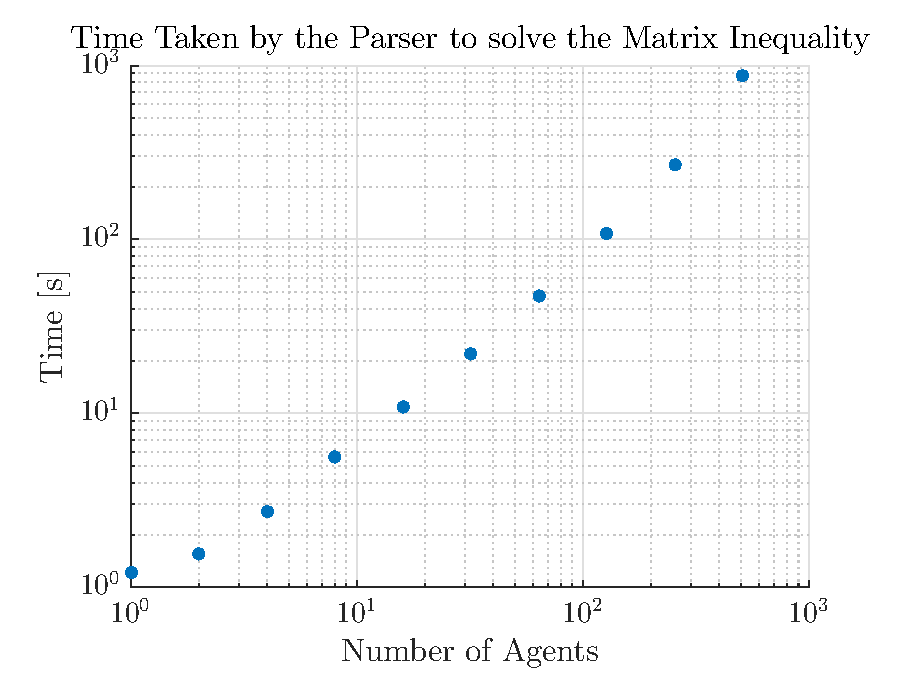
\includegraphics[width=\columnwidth]{./imgs/ParserTime}
	\caption{Time take by the parser to solve the MI \eqref{eq:MI formulation} for the three cases under consideration. The number of agents started with one system and doubled  until the maximum that the computer could process (4 for the unconstrained case, 256 for the ``neighbor'' case and 512 for the fully decentralized case). Axes are on log scale.}
	\label{fig:time graph}
\end{figure}

According to the graph shown in Figure \ref{fig:time graph}, for $N=1,2$, the time taken by the parser to solve the MI \eqref{eq:MI formulation} was of the same order of magnitude for the three cases. However, as the number of systems increases, the unconstrained case takes more time to be solved than the ``neighbor''-constrained case which, in turn, takes more time than the fully decentralized-constrained case. The time difference between the two latter cases can be explained by fact that, for the ``neighbor'' case, the matrix $Y$ contains more non-identically zero elements than the fully decentralized case. In addition to this, in the former case, each element is defined as a polynomial of second degree on the variables $q_i$ and $\breve{q}_i$, while for the latter, they are defined on the variable $q_i$ only.

Regarding the on-line integration phase, since the matrices $W$ computed in each case is  constant, for each index $i\in\mathbb{N}_{[1,4]}$, the geodesic curve connecting the origin to a point $q_i\in\mathbb{R}^2$ is a straight line: $\gamma_i(s)=sq_i$, where $s\in[0,1]$. For each case, and for each index $i\in\mathbb{N}_{[1,4]}$, the feedback law is  given by the formula
\begin{equation*}
	k= \int_0^1Y(sq)W^{-1}q\,ds.
\end{equation*}
Given the structure of the matrices $Y$ and $W$, each line $i\in\mathbb{N}_{[1,4]}$ is given by
\begin{equation*}
k_i=\begin{cases}
	\displaystyle\int_0^1Y_i(sq)W_i^{-1}q_i\,ds,&\text{if unconstrained}\\
	\displaystyle\int_0^1Y_i(sq_i,s\breve{q}_i)W_i^{-1}q_i\,ds,&\text{if ``neighbor''}\\
	\displaystyle\int_0^1Y_i(sq_i)W_i^{-1}q_i\,ds,&\text{if fully decentralized.}
\end{cases}
\end{equation*}
Moreover, from Theorem~\ref{thm:main result}, the feedback law $k$ solves Problem~\ref{problem formulation} for the network resulting from the interconnection of systems \eqref{eq:example}.


\section{Conclusion}\label{sec:Conclusion}

In this work, input-affine nonlinear systems were considered. The problem was the design of structured feedback laws. The methodology employed for synthesis was based on control-contraction metrics which provides a controller ensuring exponential convergence of pairs of solutions.

In terms of dynamic programming, employing control-contraction metrics allows one to formulate the search for the controller as a convex optimization problem. Although this is one of its main advantages over the search of control-Lyapunov functions, it does not scale well.

For systems described by a non-fully connected graph, the approach presented in this paper exploits sparsity to design feedback laws with a prescribed structure. More precisely, by imposing a block-diagonal structure on the matrix describing the metric, a controller with a prescribed structure can be synthesized. Moreover, the on-line integration phase computation can be in parallel, because each block defines a metric to the corresponding component of the state space where the geodesic is computed by optimization.

\appendices


% Can use something like this to put references on a page
% by themselves when using endfloat and the captionsoff option.
\ifCLASSOPTIONcaptionsoff
  \newpage
\fi



% trigger a \newpage just before the given reference
% number - used to balance the columns on the last page
% adjust value as needed - may need to be readjusted if
% the document is modified later
%\IEEEtriggeratref{8}
% The "triggered" command can be changed if desired:
%\IEEEtriggercmd{\enlargethispage{-5in}}

% references section

% can use a bibliography generated by BibTeX as a .bbl file
% BibTeX documentation can be easily obtained at:
% http://mirror.ctan.org/biblio/bibtex/contrib/doc/
% The IEEEtran BibTeX style support page is at:
% http://www.michaelshell.org/tex/ieeetran/bibtex/
%\bibliographystyle{IEEEtran}
% argument is your BibTeX string definitions and bibliography database(s)
%\bibliography{IEEEabrv,../bib/paper}
%
% <OR> manually copy in the resultant .bbl file
% set second argument of \begin to the number of references
% (used to reserve space for the reference number labels box)
\printbibliography


\end{document}


